\documentclass[../AnalysisNoteJBuxton.tex]{subfiles}


\begin{document}

\subsubsection{Results: \texorpdfstring{$\Lambda$K$^{0}_{S}$ and $\Lambda$K$^{\pm}$: Fit Method Comparisons}{TEXT}}
\label{ResultsLamK_FitMethComp}

In Figure \ref{fig:FitResults_ShareR_Sharelam_PolyBgd}, we show extracted fit parameters for the case of \LamKchPALamKchM sharing radii with \LamKchMALamKchP.  The figure shows results for three different treatments of the non-femtoscopic background: a polynomial fit to THERMINATOR 2 simulation to model the background (circles), a linear fit to the data to model the background (squares), and the Stavinsky method (crosses).


\begin{figure}[h]
  \centering
  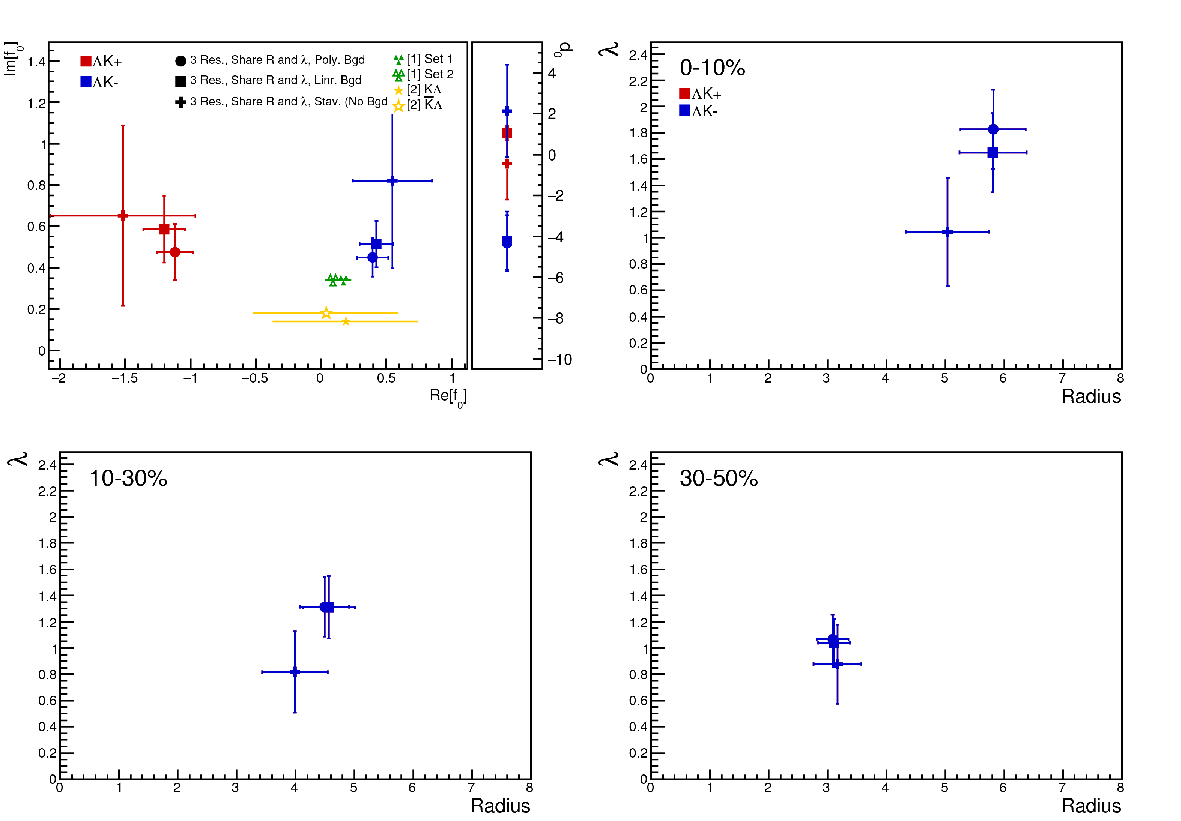
\includegraphics[width=\textwidth]{7_ResultsAndDiscussion/Figures/CompareAllScattParams_ShareR_Sharelam.pdf}
  \caption[Fit Results: Shared Radii and THERMINATOR 2 Background]{Extracted fit results for all of our \LamALamKpm systems across all studied centrality bins (0-10\%, 10-30\%, 30-50\%).  The \LamKchPALamKchM and \LamKchMALamKchP systems share both a radius and a $\lambda$ parameter for each centrality bin (i.e. 3 total radius parameters, 3 total $\lambda$ parameters).  The figure shows results for three different treatments of the non-femtoscopic background: a polynomial fit to THERMINATOR 2 simulation to model the background (circles), a linear fit to the data to model the background (squares), and the Stavinsky method (crosses).  Note, \LamKchP on the plot is shorthand for \LamKchP and \ALamKchM (\LamKchPALamKchM), and similar for the others.  The green \cite{Liu:2006xja} and yellow \cite{Mai:2009ce} points show theoretical predictions made using chiral perturbation theory.}
  \label{fig:FitResults_ShareR_Sharelam_PolyBgd}
\end{figure}


\begin{figure}[h]
  \centering
  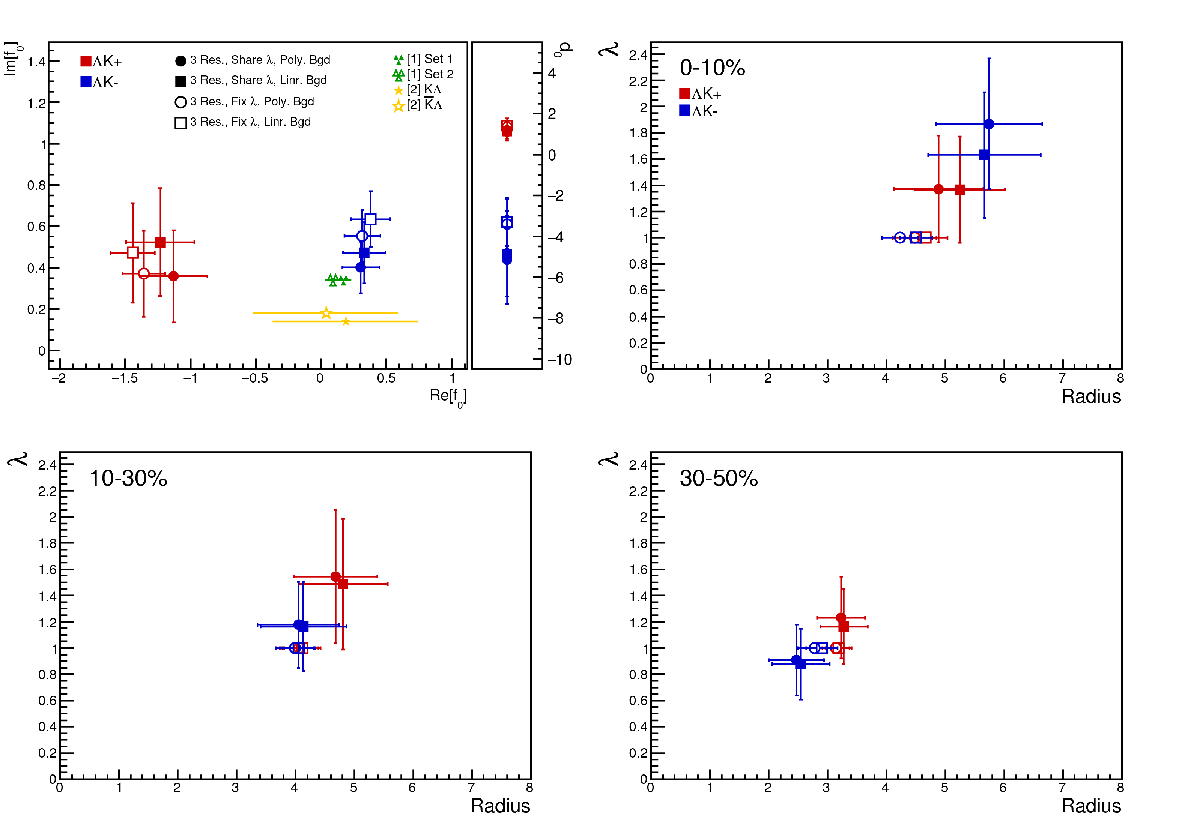
\includegraphics[width=\textwidth]{7_ResultsAndDiscussion/Figures/CompareAllScattParams_FreevsFixlam_SepR_NoStav.pdf}
  \caption[Compare Fit Parameters: Free vs fixed $\lambda$]{Compare Fit Parameters: Free vs fixed $\lambda$}
  \label{fig:CompareAllScattParams_FreevsFixlam_SepR_NoStav}
\end{figure}

\begin{figure}[h]
  \centering
  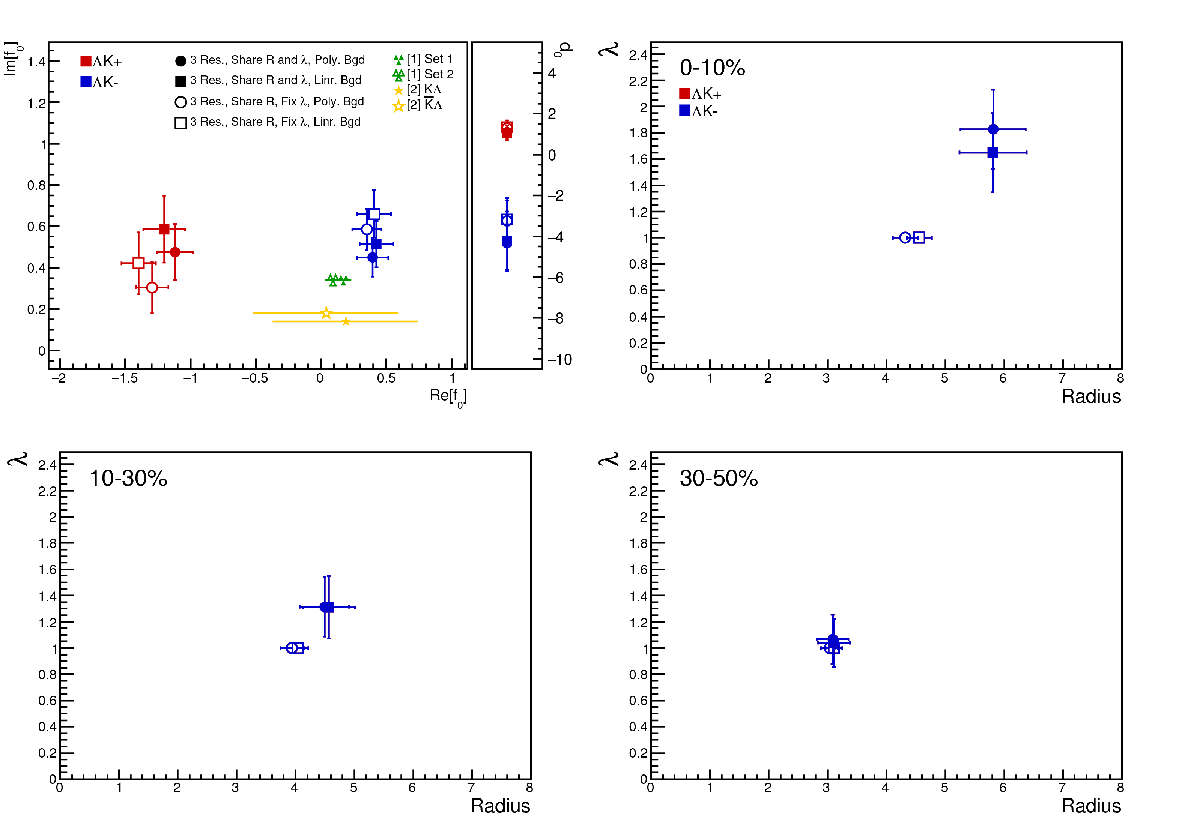
\includegraphics[width=\textwidth]{7_ResultsAndDiscussion/Figures/CompareAllScattParams_FreevsFixlam_ShareR_NoStav.pdf}
  \caption[Compare Fit Parameters: Free vs fixed $\lambda$ (sharing radii)]{Compare Fit Parameters: Free vs fixed $\lambda$ (sharing radii)}
  \label{fig:CompareAllScattParams_FreevsFixlam_ShareR_NoStav}
\end{figure}

\begin{figure}[h]
  \centering
  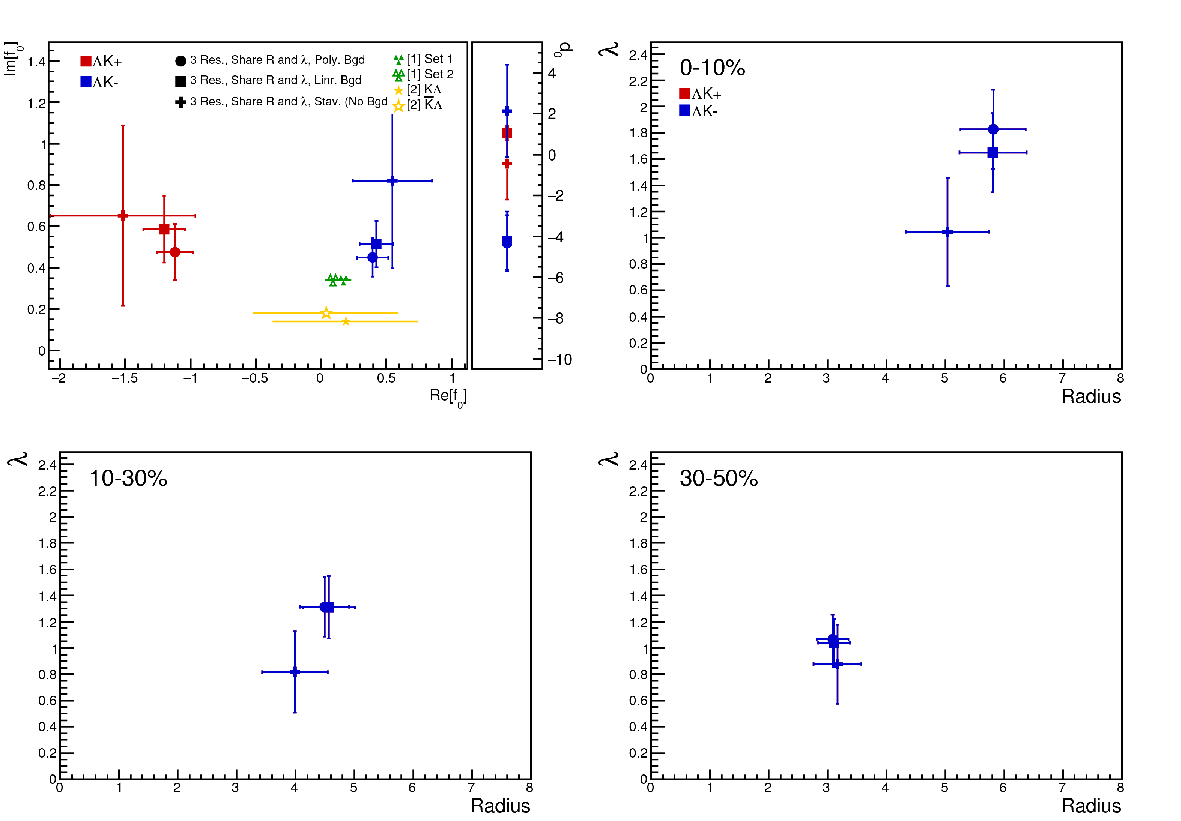
\includegraphics[width=\textwidth]{7_ResultsAndDiscussion/Figures/CompareAllScattParams_ShareR_Sharelam.pdf}
  \caption[Compare Fit Parameters: Background methods (sharing radii)]{Compare Fit Parameters: Background methods (sharing radii)}
  \label{fig:CompareAllScattParams_ShareR_Sharelam}
\end{figure}

\begin{figure}[h]
  \centering
  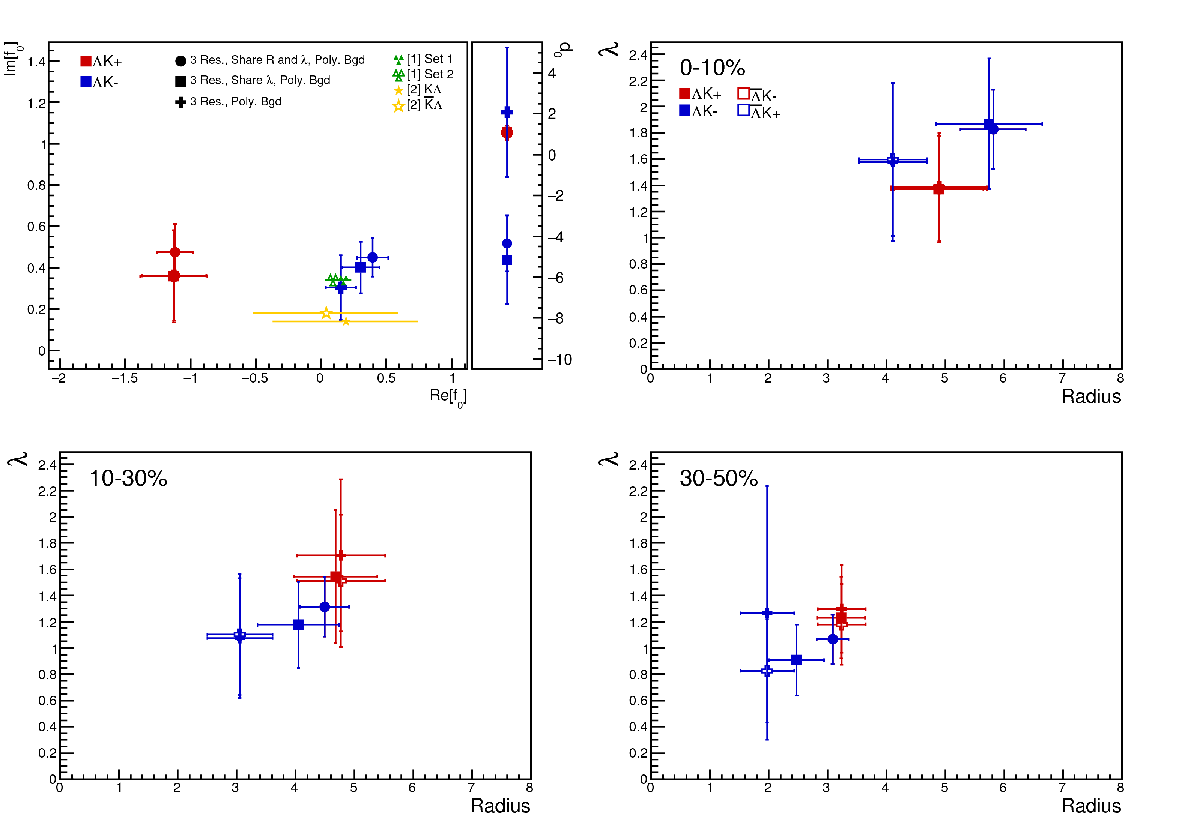
\includegraphics[width=\textwidth]{7_ResultsAndDiscussion/Figures/CompareAllScattParams_SharevsSepR.pdf}
  \caption[Compare Fit Parameters: Shared vs. Separate Radii]{Compare Fit Parameters: Shared vs. Separate Radii}
  \label{fig:CompareAllScattParams_SharevsSepR}
\end{figure}

\end{document}